\documentclass[11pt,a4paper]{article}

\usepackage[T1]{fontenc}
\usepackage{lmodern}
\usepackage[utf8]{inputenc}
\usepackage[margin=2.5cm]{geometry}
\usepackage{booktabs}
\usepackage{graphicx}
\usepackage{amsmath}
\usepackage{caption}
\usepackage[colorlinks=true,allcolors=black]{hyperref}
\usepackage{microtype}

\captionsetup{font=small,labelfont=bf}
\setlength{\parskip}{0.35em}

\title{\large Graph-level supervision, not node-level self-supervision,\\
improves low-label molecular property prediction under scaffold splits}

\author{Nguyen Ngoc Dung}
\date{September 2026}

\begin{document}
\maketitle

\begin{abstract}
\noindent
Self-supervised pretraining is widely reported to improve molecular property
prediction where labelled data are scarce, yet reported gains are frequently
small relative to the variation introduced by seed and split selection. Whether
such pretraining confers a genuine advantage therefore depends on the rigour of
the evaluation applied to it. We evaluate node-level and graph-level pretraining
on the Tox21 toxicity benchmark under a protocol fixed before any measurement:
Bemis--Murcko scaffold splits that place unseen molecular frameworks in the test
partition, pretraining corpora decontaminated against every held-out scaffold,
repeated seeds at each level of supervision, and decision thresholds specified
in advance. A complete two-factor design separates the contribution of each
pretraining level and allows their interaction to be estimated rather than
assumed. Node-level self-supervision yields no improvement distinguishable from
seed variation, whereas graph-level supervised pretraining improves prediction
at every level of supervision examined, with the largest advantage where
labelled data are most limited. The two levels contribute additively, and no
synergy between them is detectable. Substituting a random split for a scaffold
split inflates the same benchmark by more than any pretraining effect this study
measures, indicating that the evaluation protocol governs the conclusion more
strongly than the choice of pretraining objective. Code is available at:
\url{https://github.com/ngocdung03/mol-ssl}
\end{abstract}

\section{Introduction}

Labelled molecular property data are costly to obtain, and pretraining on
unlabelled or auxiliary corpora is the standard response. Reported gains are
frequently modest relative to the variation induced by seed and split choice,
which makes the evaluation protocol a determinant of the reported effect rather
than a neutral background.

Hu et al.~\cite{hu2020} distinguish two levels at which a graph neural network
may be pretrained. Node-level objectives, such as attribute masking, regularise
individual atom representations; graph-level objectives fit a supervised
multi-task head on pooled graph representations. Their central observation is
that strategies operating at only one level yield limited improvement and can
produce negative transfer, whereas the two levels applied in sequence perform
best. Their reported averages across eight MoleculeNet datasets are $67.0$
ROC-AUC without pretraining, $71.4$ for node-level attribute masking, $68.9$ for
graph-level supervision alone, and $73.5$ for the two combined.

The present study asks whether that ordering reproduces on a single dataset
under an evaluation protocol designed to make small effects distinguishable from
noise, and separates the contribution of each level using a complete two-factor
design.

\section{Methods}

\subsection{Evaluation protocol}

All splits are Bemis--Murcko scaffold splits at proportions $0.8/0.1/0.1$,
generated once and stored as a manifest that the training code loads rather than
recomputes. The Tox21 dataset comprises $7{,}823$ molecules across twelve assay
tasks, partitioned into $6{,}258$ training, $782$ validation and $783$ test
molecules. The split is deterministic and independent of seed, so the seed
varies only the labelled subsample and the model initialisation. Random splits
are not available to the training path; they are confined to a separate
comparison module used solely for the inflation measurement in
Section~\ref{sec:inflation}.

Model selection uses the validation partition. The test partition is evaluated
once, at the end of training, using the validation-selected parameters. The
reported epoch is the early-stopping epoch and never the epoch of best test
performance. Every reported quantity is a mean and sample standard deviation
over the five seeds $\{0,1,2,3,4\}$.

\subsection{Model and objectives}

The encoder is a five-layer GINE network with $300$ hidden units, batch
normalisation, dropout $0.1$, and mean pooling as the readout. The prediction
head is a single linear layer over the pooled representation, with twelve
outputs for Tox21. The loss masks unobserved labels; a missing assay is not
treated as a negative.

Two pretraining objectives were implemented behind a common interface.
Node-level attribute masking zeroes the atom-type block of a randomly selected
$15\%$ of atoms and reconstructs the hidden element from the surrounding graph
context. Graph-level supervision fits a linear head on the pooled graph
representation against $128$ PCBA bioassays under the same masked loss. Only
encoder parameters transfer to the downstream task; both pretraining heads are
discarded.

\subsection{Factorial design}

Node-level and graph-level pretraining were treated as two binary factors,
giving four conditions that differ only in the encoder parameters at the start of
fine-tuning:

\begin{center}
\small
\begin{tabular}{lll}
\toprule
 & graph-level absent & graph-level present \\
\midrule
node-level absent  & \texttt{none}: random initialisation & \texttt{graph}: PCBA supervision \\
node-level present & \texttt{node}: attribute masking     & \texttt{node\_graph}: masking, then PCBA \\
\bottomrule
\end{tabular}
\end{center}

The combined condition applies the two stages in the order specified by
Hu et al.: node-level self-supervision first, then graph-level supervision
initialised from the resulting encoder. Splits, seeds, labelled subsamples,
optimiser and learning rate are identical across all four conditions. A single
fixed fine-tuning learning rate was used for every condition; tuning one
condition and not another is a recognised route to a spurious difference.

\subsection{Corpus decontamination}

Node-level pretraining used ZINC250k. Of $249{,}455$ molecules, $10{,}335$
($4.14\%$) shared a Bemis--Murcko scaffold with a downstream validation or test
partition and were removed, leaving $239{,}120$. Graph-level pretraining used
PCBA. Of $437{,}927$ molecules, $18{,}809$ ($4.30\%$) were removed on the same
criterion, leaving $419{,}118$. Filtering was applied against the held-out
scaffolds of all four downstream manifests, comprising $1{,}565$ scaffolds for
Tox21 and $3{,}116$ in total.

The filter is re-applied at the start of every pretraining run rather than
trusted from the cached corpus, and a run whose corpus fails the check is
refused. A negative control in which ten Tox21 validation and test molecules
were inserted into a corpus was rejected with a non-zero exit status and no
checkpoint written. The regression test for the filter is verified by mutation:
disabling the filter body causes the test to fail, so a test that cannot fail is
not accepted as evidence.

\subsection{Pre-registered analysis}

Hypotheses and thresholds were recorded before the sweep was executed. The
following ordering was predicted from Hu et al.:
\begin{center}
\texttt{node\_graph} $>$ \texttt{node} $>$ \texttt{graph} $>$ \texttt{none}.
\end{center}

A single primary comparison was nominated in advance: \texttt{node\_graph}
against \texttt{none} at full supervision. For the remaining fifteen
comparisons, a condition is declared to exceed noise only when
$|\Delta| > 2\sigma_{\mathrm{pooled}}$, where $\sigma_{\mathrm{pooled}}$ is the
root sum of squares of the two seed standard deviations. The unadjusted
criterion $|\Delta| > \sigma_{\mathrm{pooled}}$ is reported alongside for
continuity with earlier work on the same benchmark. The interaction contrast
\begin{equation}
\Delta_{\mathrm{int}}
= (\texttt{node\_graph} - \texttt{graph}) - (\texttt{node} - \texttt{none})
= \texttt{node\_graph} - (\texttt{graph} + \texttt{node}) + \texttt{none}
\label{eq:int}
\end{equation}
was specified as the test of whether the two levels combine additively. This
contrast is introduced in the present study; the two-factor layout follows
Hu et al., whose analysis is comparative and does not evaluate an interaction.

\section{Results}

\subsection{Split-induced inflation}
\label{sec:inflation}

An identical model trained on identical data, differing only in the partitioning
rule, attained $0.7383 \pm 0.0070$ AUROC under a scaffold split and
$0.8226 \pm 0.0146$ under a random split. The inflation is
$0.0843 \pm 0.0140$ AUROC and was positive on all five seeds. This magnitude
exceeds every pretraining effect reported below and establishes the scale
against which those effects should be read.

\subsection{The node by graph factorial}

Both pretraining stages converged. Node-level masking loss decreased from
$0.1518$ to $0.0338$ over twenty epochs on $239{,}120$ molecules. Graph-level
assay loss decreased to $0.0364$ from random initialisation and to $0.0352$ when
initialised from the node-level encoder. The three pretrained encoders were
confirmed pairwise distinct, so no two conditions represent the same parameters
under different labels.

\begin{table}[htbp]
\centering
\small
\caption{Test AUROC on Tox21 under a Bemis--Murcko scaffold split, mean and
sample standard deviation over five seeds. Run \texttt{0903\_1750\_tox21\_2x2\_full};
four conditions at five labelled fractions, $100$ fine-tuning runs.}
\label{tab:main}
\begin{tabular}{rrcccc}
\toprule
Labelled fraction & $n_{\mathrm{train}}$ & \texttt{none} & \texttt{node} & \texttt{graph} & \texttt{node\_graph} \\
\midrule
5\%   & 313  & $0.6215 \pm 0.0442$ & $0.6368 \pm 0.0277$ & $0.6745 \pm 0.0208$ & $0.6936 \pm 0.0307$ \\
10\%  & 626  & $0.6253 \pm 0.0291$ & $0.6631 \pm 0.0316$ & $0.6970 \pm 0.0196$ & $0.7168 \pm 0.0118$ \\
25\%  & 1,564 & $0.6937 \pm 0.0114$ & $0.6879 \pm 0.0181$ & $0.7229 \pm 0.0080$ & $0.7300 \pm 0.0138$ \\
50\%  & 3,129 & $0.7083 \pm 0.0198$ & $0.7194 \pm 0.0073$ & $0.7502 \pm 0.0074$ & $0.7554 \pm 0.0120$ \\
100\% & 6,258 & $0.7293 \pm 0.0063$ & $0.7505 \pm 0.0106$ & $0.7571 \pm 0.0120$ & $0.7676 \pm 0.0179$ \\
\bottomrule
\end{tabular}
\end{table}

Table~\ref{tab:main} and Figure~\ref{fig:curve} report the four conditions. The
combined condition attained the highest value at every labelled fraction.
Table~\ref{tab:delta} reports the corresponding differences from random
initialisation.

\begin{table}[htbp]
\centering
\small
\caption{Differences in AUROC from random initialisation. Marks denote the
pre-registered criteria: $\ast$ exceeds $\sigma_{\mathrm{pooled}}$;
$\ast\ast$ exceeds $2\sigma_{\mathrm{pooled}}$; unmarked entries lie inside
seed noise.}
\label{tab:delta}
\begin{tabular}{rccc}
\toprule
Labelled fraction & \texttt{node} & \texttt{graph} & \texttt{node\_graph} \\
\midrule
5\%   & $+0.0154$          & $+0.0530^{\ast}$   & $+0.0722^{\ast}$ \\
10\%  & $+0.0377$          & $+0.0716^{\ast\ast}$ & $+0.0914^{\ast\ast}$ \\
25\%  & $-0.0058$          & $+0.0292^{\ast\ast}$ & $+0.0363^{\ast\ast}$ \\
50\%  & $+0.0110$          & $+0.0419^{\ast}$   & $+0.0470^{\ast\ast}$ \\
100\% & $+0.0212^{\ast}$   & $+0.0278^{\ast\ast}$ & $+0.0384^{\ast\ast}$ \\
\midrule
Fractions exceeding $\sigma_{\mathrm{pooled}}$  & 1 of 5 & 5 of 5 & 5 of 5 \\
Fractions exceeding $2\sigma_{\mathrm{pooled}}$ & 0 of 5 & 3 of 5 & 4 of 5 \\
\bottomrule
\end{tabular}
\end{table}

\begin{figure}[htbp]
\centering
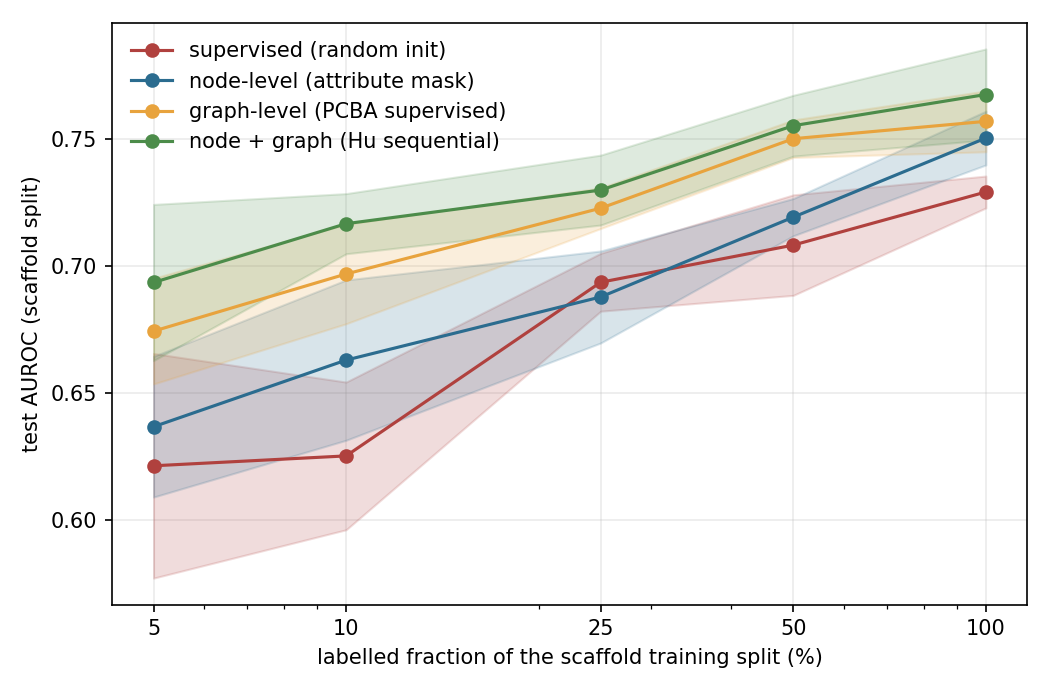
\includegraphics[width=0.86\textwidth]{fig_labelled_fraction.png}
\caption{Test AUROC on Tox21 against the labelled fraction of the scaffold
training split, for the four pretraining conditions. Bands span one sample
standard deviation.}
\label{fig:curve}
\end{figure}

Three observations follow. First, node-level pretraining alone satisfied the
adjusted criterion at none of the five labelled fractions, and at a labelled fraction of 25\% its
difference was negative. Second, graph-level pretraining satisfied the
unadjusted criterion at all five labelled fractions and the adjusted criterion at three.
Third, the primary pre-specified comparison, \texttt{node\_graph} against
\texttt{none} at full supervision, gave $+0.0384$ with
$\sigma_{\mathrm{pooled}} = 0.0190$ and satisfied the adjusted criterion; being
nominated in advance, it requires no multiplicity adjustment.

The advantage of the combined condition increased as supervision was reduced,
from $+0.0384$ at full supervision to $+0.0722$ at a labelled fraction of 5\%. The
\texttt{node} column was measured five weeks after an independent sweep of the
same condition and agreed with it within $\sigma_{\mathrm{pooled}}$ at every
labelled fraction, the largest discrepancy being $0.0096$.

\subsection{Interaction}

The contrast of Equation~\ref{eq:int} took the values $+0.0038$, $-0.0179$,
$+0.0129$, $-0.0059$ and $-0.0107$ at the five labelled fractions, against pooled standard
deviations of $0.0640$, $0.0486$, $0.0267$, $0.0254$ and $0.0248$. Every value
lies inside seed noise and the sign alternates. The two objectives therefore
contribute additively, with no detectable synergy.

Applying the same contrast to the averages of Hu et al. gives
$73.5 - (68.9 + 71.4) + 67.0 = +0.2$, also consistent with additivity. Their
result rests on two positive main effects that accumulate, rather than on an
interaction between them. The present finding is therefore consistent with their
data on this point.

\section{Discussion}

The ordering of the two main effects is reversed relative to Hu et al. In their
averages, graph-level supervision alone was nearly inert, at $68.9$ against a
baseline of $67.0$, with negative transfer on two of eight datasets, and
node-level masking carried most of the improvement. In the present study,
graph-level supervision accounted for the larger part of the effect and
node-level masking contributed little.

Several differences between the two studies could account for this reversal, and
all are hypotheses rather than results. Scale is the most probable: Hu et al.
pretrained at the node level on two million ZINC15 molecules, against $239{,}120$
after decontamination in the present study, leaving the node-level encoder
correspondingly less well trained. The graph-level corpora differ in kind, their
ChEMBL panel spanning $1{,}310$ broad biochemical assays against the $128$
bioactivity screens of PCBA, which plausibly resemble the twelve Tox21 endpoints
more closely and so transfer more effectively. Their figures are means over
eight datasets, from which one dataset may depart without contradicting them;
attribute masking produced negative transfer on ToxCast in their own results.
Decontamination was asymmetric, their Section 5.1 filtering only the graph-level
corpus while both corpora were filtered in the present study. The encoders also
differ, theirs a GIN with integer atom-type embeddings against a GINE with
continuous atom features and per-layer edge features.

A second observation concerns the interpretation of published gains. A standard
pretraining corpus contained $4.30\%$ of molecules sharing a scaffold with the
downstream evaluation partitions. A pipeline that omits this filter pretrains on
evaluation chemotypes, and the resulting difference cannot be attributed to
transfer. Combined with the inflation of $0.0843$ AUROC obtained by substituting
a random split, this indicates that protocol choices span a range wider than the
effects under study.

\subsection*{Limitations}

The graph-level corpus is PCBA, comprising $437{,}927$ molecules and $128$ assays,
in place of the ChEMBL corpus of Hu et al., which contains approximately
$456{,}000$ molecules and $1{,}310$ assays. Molecule counts are comparable; task
breadth is approximately one tenth. The node-level corpus is smaller by a larger
margin: $239{,}120$ decontaminated ZINC250k molecules against the two million
ZINC15 molecules of Hu et al. The node-level condition is therefore
under-trained relative to theirs, and the absence of a measurable node-level
effect in this study should not be read as evidence that the objective is
ineffective at scale. Evaluation is restricted to Tox21, so the
generality of the reversed main effects is untested, and the proposed
resemblance between the graph-level corpus and the downstream endpoints cannot
be examined. One node-level objective was implemented;
context prediction, edge prediction and contrastive objectives were not.
Pretraining ran for twenty epochs at each stage, a schedule that was not tuned.
The threshold at $2\sigma_{\mathrm{pooled}}$ is a pragmatic guard against
multiplicity and not a hypothesis test; paired per-seed tests or a mixed model
over seeds and labelled fractions would be preferable. The corpus was filtered against all
four downstream manifests rather than Tox21 alone, which is mildly unfavourable
to the graph-level conditions.

\begin{thebibliography}{9}
\small
\bibitem{hu2020}
W.~Hu, B.~Liu, J.~Gomes, M.~Zitnik, P.~Liang, V.~Pande, and J.~Leskovec.
Strategies for pre-training graph neural networks.
\textit{International Conference on Learning Representations}, 2020.
arXiv:1905.12265.

\bibitem{wu2018}
Z.~Wu, B.~Ramsundar, E.~N.~Feinberg, J.~Gomes, C.~Geniesse, A.~S.~Pappu,
K.~Leswing, and V.~Pande.
MoleculeNet: a benchmark for molecular machine learning.
\textit{Chemical Science}, 9(2):513--530, 2018.

\bibitem{xu2019}
K.~Xu, W.~Hu, J.~Leskovec, and S.~Jegelka.
How powerful are graph neural networks?
\textit{International Conference on Learning Representations}, 2019.

\bibitem{bemis1996}
G.~W.~Bemis and M.~A.~Murcko.
The properties of known drugs. 1. Molecular frameworks.
\textit{Journal of Medicinal Chemistry}, 39(15):2887--2893, 1996.
\end{thebibliography}

\end{document}
